
\hypertarget{menu_r}{}
\section{R}
\index{R menu}

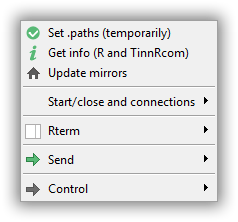
\includegraphics[scale=0.8]{./res/menu_r.png}\\

\begin{scriptsize}
  \begin{tabularx}{\textwidth}{>{\hsize=0.5\hsize}X>{\hsize=0.7\hsize}X}\\
    \hline
    \textbf{Option} & \textbf{Description} \\
    \hline
    Set .paths (temporarily) & Sets (temporarily) the necessary .paths object in \RR{} environment.
     This object provided by TinnRcom package. This option is useful only if the user can not,
     for some reason, install the TinnRcom package \\
    Get info (R and TinnRcom) & Get information about \RR{} and the necessary TinnRcom package \\
    Update mirrors & Updates the Rmirrors.xml file \\
    \hdashline[1pt/1pt]
    Toogle (start/close) & \textit{\href{\#menu\_r\_toogle\_start}{See options ...}} \\
    Toogle (active \RR{}) & \textit{\href{\#menu\_r\_toogle\_active}{See options ...}} \\
    \hdashline[1pt/1pt]
    Send & \textit{\href{\#menu\_r\_send}{See options ...}} \\
    Control & \textit{\href{\#menu\_r\_control}{See options ...}} \\
    \hdashline[1pt/1pt]
    Term & \textit{\href{\#menu\_r\_term}{See options ...}} \\
    Code completion (dlg) & Opens the dialog window for efficient search of R objects.
    \textit{\href{\#additional_dialogs_code_completion}{See more details ...}} \\
    \hline
  \end{tabularx}
\end{scriptsize}

\hypertarget{menu_r_toogle_start}{}
\subsection{Toogle (start/close)}
\index{R menu!Toogle (start/close))}

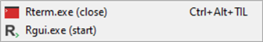
\includegraphics[scale=0.8]{./res/menu_r_toogle_start.png}\\

\begin{scriptsize}
  \begin{tabularx}{\textwidth}{>{\hsize=0.7\hsize}X>{\hsize=0.7\hsize}X}\\
    \hline
    \textbf{Option} & \textbf{Description} \\
    \hline
    Rterm.exe (start/close) & Toggles Rterm.exe \\
    Rgui.exe (start/close) & Toggles Rgui.exe \\
    \hline
  \end{tabularx}
\end{scriptsize}

\hypertarget{menu_r_toogle_active}{}
\subsection{Toogle (active \RR{})}
\index{R menu!Toogle (active R))}

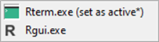
\includegraphics[scale=0.8]{./res/menu_r_toogle_active.png}\\

\begin{scriptsize}
  \begin{tabularx}{\textwidth}{>{\hsize=0.7\hsize}X>{\hsize=0.7\hsize}X}\\
    \hline
    \textbf{Option} & \textbf{Description} \\
    \hline
    Rterm.exe & (is set as active*) \\
    Rgui.exe \\
    \hline
  \end{tabularx}
\end{scriptsize}

\hypertarget{menu_r_send}{}
\subsection{Send}
\index{R menu!send}

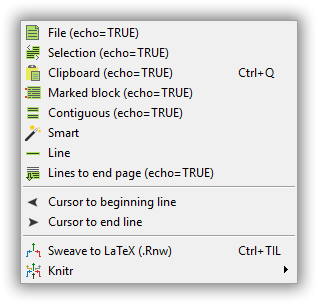
\includegraphics[scale=0.8]{./res/menu_r_send.png}\\

\begin{scriptsize}
  \begin{tabularx}{\textwidth}{>{\hsize=0.5\hsize}X>{\hsize=0.7\hsize}X}\\
    \hline
    \textbf{Option} & \textbf{Description} \\
    \hline
    File & Sends current file to R interpreter \\
    Selection & Sends current selection to R interpreter \\
    Marked block & Sends current marked block to R interpreter \\
		  Contiguous & Sends contiguous lines to R interpreter \\
    %Smart & Sends complete instruction blocks when the cursor is located in a complex context \\
    Line & Sends current line to R interpreter echoing it \\
    Lines to end page & Sends all visible lines to end page echoing it \\
    \hdashline[1pt/1pt]
    Cursor to beginning line & Sends cursor position to beginning line \\
    Cursor to end line & Sends cursor position to end line \\
    \hdashline[1pt/1pt]
    Sweave & Sends to R interpreter \texttt{Sweave('Active file')} instruction \\
    Knitr & \textit{\href{\#menu\_r\_send\_knitr}{See options ...}} \\
    \hline
  \end{tabularx}
\end{scriptsize}

\hypertarget{menu_r_send_knitr}{}
\subsubsection{Knitr:}\\
\index{Knitr}

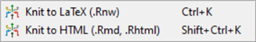
\includegraphics[scale=0.8]{./res/menu_r_send_knitr.png}\\

\begin{scriptsize}
  \begin{tabularx}{\textwidth}{>{\hsize=0.3\hsize}X>{\hsize=0.7\hsize}X}\\
    \hline
    \textbf{Option} & \textbf{Description} \\
    \hline
    Knit to \LaTeX ~(Rnw) & Knit the *.Rnw file to \LaTeX \\
    Knit to HTML (Rmd, Rhtml) & Knit the *.Rmd or *.Rhtml file to HTML \\
    \hline
  \end{tabularx}
\end{scriptsize}

\hypertarget{menu_r_control}{}
\subsection{Control}
\index{R menu!control}

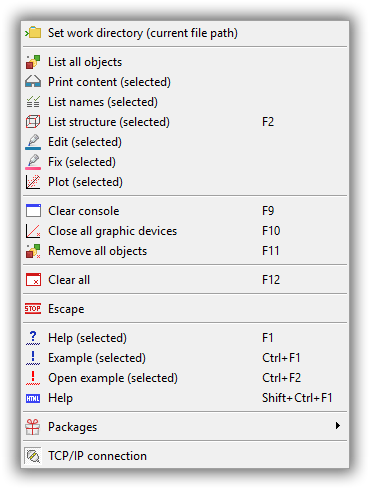
\includegraphics[scale=0.8]{./res/menu_r_control.png}\\

\begin{scriptsize}
  \begin{tabularx}{\headwidth}{>{\hsize=0.4\hsize}X>{\hsize=0.7\hsize}X}\\
    \hline
    \textbf{Option} & \textbf{Description} \\
    \hline
    Work directory (get/set) &  \textit{\href{\#menu\_r\_control\_workdir}{See options ...}} \\
    \hdashline[1pt/1pt]
    List all objects & Sends to R interpreter a \texttt{ls()} instruction \\
    Content (selected) & Sends to R interpreter a \texttt{selected} word \\
    List names (selected) & Sends to R interpreter a \texttt{names(selected)} instruction \\
    List structure (selected) & Sends to R interpreter a \texttt{str(selected)} instruction \\
    Edit (selected) & Sends to R interpreter a \texttt{edit(selected)} instruction \\
    Fix (selected) & Sends to R interpreter a \texttt{fix(selected)} instruction \\
    Plot (selected) & Sends to R interpreter a \texttt{plot(selected)} instruction \\
    \hdashline[1pt/1pt]
    Clear console & Sends and executes the virtual \texttt{CTRL + L} (clear screen) instruction \\
    Close all graphic devices & Sends to R interpreter a \texttt{graphics.off()} instruction \\
    Remove all objects & Sends to R interpreter a \texttt{rm(list=ls())} instruction \\
    \hdashline[1pt/1pt]
    Clear all & Sends to R interpreter a \texttt{graphics.off()}; \texttt{rm(list=ls())}
     \texttt{CTRL + L} instructions \\
    \hdashline[1pt/1pt]
    Escape & Stops all computations in Rgui.exe \\
    \hdashline[1pt/1pt]
    Help (selected) & Sends to R interpreter a \texttt{help(selected)} instruction \\
    Example (selected) & Sends to R interpreter a \texttt{example(selected)} instruction \\
    Open example (selected) & Sends to R interpreter an instruction to generate an example
     text file of the \texttt{object selected}\\
    Help & Sends to R interpreter a \texttt{help.start(update=FALSE)} instruction \\
    \hdashline[1pt/1pt]
    Packages & \textit{\href{\#menu\_r\_control\_packages}{See options ...}} \\
    TCP/IP connection & Sends to R interpreter an instruction to start:
     \texttt{startSocketServer(port=portnumber)} or stop: \texttt{startSocketServer(port=portnumber)}
     the TCP/IP connection \\
    \hline
  \end{tabularx}
\end{scriptsize}

\hypertarget{menu_r_control_packages}{}
\subsubsection{Packages:}\\
\index{R menu!control packages}

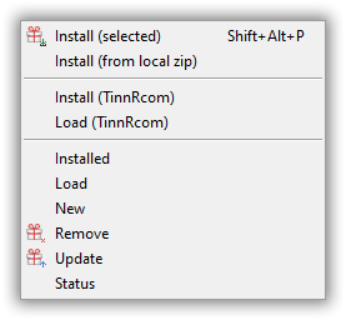
\includegraphics[scale=0.8]{./res/menu_r_control_packages.png}\\

\begin{scriptsize}
  \begin{tabularx}{\headwidth}{>{\hsize=0.2\hsize}X>{\hsize=0.7\hsize}X}\\
    \hline
    \textbf{Option} & \textbf{Description} \\
    \hline
    CRAN web page (selected) & Open the selected package page in the default browser \\
    \hdashline[1pt/1pt]
    Install (selectd) )& Sends to R interpreter an \texttt{utils:::menuInstallPkgs()} instruction \\
    Install (from local zip) & Sends to R interpreter a \texttt{utils:::menuInstallLocal()} instruction \\
    \hdashline[1pt/1pt]
    Install (TinnRcom) & Sends to R interpreter instruction to install TinnRcom package and its dependecies.
     By default it is not necessary since the TinnRcom package is automatically installed \\
    Load (TinnRcom) & Sends to R interpreter an \texttt{library(TinnRcom)} instruction.
      By default it is not necessary since the TinnRcom package is automatically loaded when R starts \\
    \hdashline[1pt/1pt]
    Require (selected) & Sends to R interpreter a \texttt{require(selected)} instruction \\
    Library (selected) & Sends to R interpreter a \texttt{library(selected)} instruction \\
    \hdashline[1pt/1pt]
    Installed & Sends to R interpreter a \texttt{installed.packages()} instruction \\
    Load & Sends to R interpreter a \texttt{local(\{pkg $<$- select.list(sort(.packages(all.available = TRUE)));
     if(nchar(pkg)) library(pkg, character.only=TRUE)\})} instruction \\
    New & Sends to R interpreter a \texttt{new.packages()} instruction \\
    Remove & Sends to R interpreter a \texttt{local(\{pkg $<$- select.list(sort(.packages(all.available = TRUE)));
     if(nchar(pkg)) remove.packages(pkg)\})} instruction \\
    Update & Sends to R interpreter an \texttt{update.packages(ask='graphics')} instruction \\
    Status & Sends to R interpreter a \texttt{packageStatus()} instruction \\
    \hline
  \end{tabularx}
\end{scriptsize}

\hypertarget{menu_r_term}{}
\subsection{Term}
\index{R menu!Term}

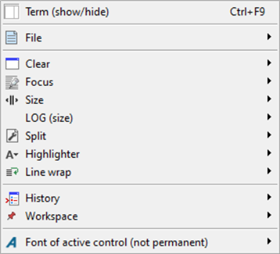
\includegraphics[scale=0.8]{./res/menu_r_term.png} \\

\begin{scriptsize}
  \begin{tabularx}{\textwidth}{>{\hsize=0.7\hsize}X>{\hsize=0.7\hsize}X}\\
    \hline
    \textbf{Option} & \textbf{Description} \\
    \hline
    Term (show/hide) & Toggles (show/hide) Term interface \\
    \hdashline[1pt/1pt]
    File & \textit{\href{\#menu\_r\_term\_file}{See options ...}} \\
    \hdashline[1pt/1pt]
    Clear & \textit{\href{\#menu\_r\_term\_clear}{See options ...}} \\
    Focus & \textit{\href{\#menu\_r\_term\_focus}{See options ...}} \\
    Size & \textit{\href{\#menu\_r\_term\_size}{See options ...}} \\
    LOG (size) &  Minimize, divide or maximize LOG \\
    Split & \textit{\href{\#menu\_r\_term\_split}{See options ...}} \\
    Highlighter & \textit{\href{\#menu\_r\_term\_highlighter}{See options ...}} \\
    Line wrap & \textit{\href{\#menu\_r\_term\_linewrap}{See options ...}} \\
    \hdashline[1pt/1pt]
    History & \textit{\href{\#menu\_r\_term\_history}{See options ...}} \\
    Workspace & \textit{\href{\#menu\_r\_term\_workspace}{See options ...}} \\
    \hdashline[1pt/1pt]
    Font of active control (not permanent) & \textit{\href{\#menu\_r\_term\_fontsize}{See options ...}} \\
    \hline
  \end{tabularx}
\end{scriptsize}

\hypertarget{menu_r_term_file}{}
\subsubsection{File:}\\
\index{R menu!Term file}

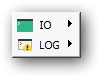
\includegraphics[scale=0.8]{./res/menu_r_term_IOandLog.png}\\

\begin{scriptsize}
  \begin{tabularx}{\textwidth}{>{\hsize=0.3\hsize}X>{\hsize=0.7\hsize}X}\\
    \hline
    \textbf{Option} & \textbf{Description} \\
    \hline
    IO & \textit{\href{\#menu\_r\_term\_file\_IO}{See options ...}} \\
    LOG & \textit{\href{\#menu\_r\_term\_file\_Log}{See options ...}} \\
    \hline
  \end{tabularx}
\end{scriptsize}

\hypertarget{menu_r_term_file_IO}{}
\subsubsection{File IO:}\\
\index{R menu!Term file IO}

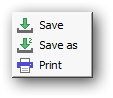
\includegraphics[scale=0.8]{./res/menu_r_term_file_IOandLog.png}\\

\begin{scriptsize}
  \begin{tabularx}{\textwidth}{>{\hsize=0.3\hsize}X>{\hsize=0.7\hsize}X}\\
    \hline
    \textbf{Option} & \textbf{Description} \\
    \hline
    Save & Saves the content of the IO interface \\
    Save as & Saves the content of the IO interface as a new file \\
    Print & Opens the Tinn-R print dialog with the content from the IO interface \\
    \hline
  \end{tabularx}
\end{scriptsize}

%\newpage
\hypertarget{menu_r_term_file_Log}{}
\subsubsection{File LOG:}\\
\index{R menu!Term file lOG}

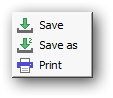
\includegraphics[scale=0.8]{./res/menu_r_term_file_IOandLog.png}\\

\begin{scriptsize}
  \begin{tabularx}{\textwidth}{>{\hsize=0.3\hsize}X>{\hsize=0.7\hsize}X}\\
    \hline
    \textbf{Option} & \textbf{Description} \\
    \hline
    Save & Saves the content of the LOG interface \\
    Save as & Saves as the content of the LOG interface \\
    Print & Opens the Tinn-R print dialog with content from LOG interface \\
    \hline
  \end{tabularx}
\end{scriptsize}

\hypertarget{menu_r_term_clear}{}
\subsubsection{Clear:}\\
\index{R menu!Term clear}

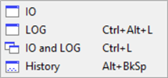
\includegraphics[scale=0.8]{./res/menu_r_term_clear.png}\\

\begin{scriptsize}
  \begin{tabularx}{\textwidth}{>{\hsize=0.3\hsize}X>{\hsize=0.7\hsize}X}\\
    \hline
    \textbf{Option} & \textbf{Description} \\
    \hline
    IO & Clear IO \\
    LOG & Clear LOG \\
    IO and LOG & Clear IO and LOG \\
    \hline
  \end{tabularx}
\end{scriptsize}

\hypertarget{menu_r_term_focus}{}
\subsubsection{Focus:}\\
\index{R menu!Term focus}

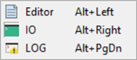
\includegraphics[scale=0.8]{./res/menu_r_term_focus.png}\\

\begin{scriptsize}
  \begin{tabularx}{\textwidth}{>{\hsize=0.3\hsize}X>{\hsize=0.7\hsize}X}\\
    \hline
    \textbf{Option} & \textbf{Description} \\
    \hline
    Editor & Places the focus inside of the \textit{editor} \\
    IO & Places the focus inside of the \textit{IO} \\
    LOG & Places the focus inside of the \textit{LOG} \\
    \hline
  \end{tabularx}
\end{scriptsize}

\hypertarget{menu_r_term_size}{}
\subsubsection{Size:}\\
\index{R menu!Term size}

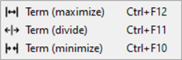
\includegraphics[scale=0.8]{./res/menu_r_term_size.png}\\

\begin{scriptsize}
  \begin{tabularx}{\textwidth}{>{\hsize=0.3\hsize}X>{\hsize=0.7\hsize}X}\\
    \hline
    \textbf{Option} & \textbf{Description} \\
    \hline
    Term (maximize) & Maximizes the Term interface \\
    Term (divide) & Divides the Term interface \\
    Term (minimize) & Minimizes the Term interface \\
    \hline
  \end{tabularx}
\end{scriptsize}

%\newpage
\hypertarget{menu_r_term_split}{}
\subsubsection{Split:}\\
\index{R menu!Term split}

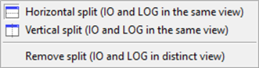
\includegraphics[scale=0.8]{./res/menu_r_term_split.png}\\

\begin{scriptsize}
  \begin{tabularx}{\headwidth}{>{\hsize=0.6\hsize}X>{\hsize=0.7\hsize}X}\\
    \hline
    \textbf{Option} & \textbf{Description} \\
    \hline
    Horizontal split (IO and LOG in the same view) & Splits horizontally the Term interface
     placing \textit{IO} and \textit{LOG} on the same view \\
    Vertical split (IO and LOG in the same view) & Splits vertically the Term interface
     placing \textit{IO} and \textit{LOG} on the same view \\
    Remove split (IO and LOG in distinct view) & Removes split placing
     \textit{IO} and \textit{LOG} in distinct view \\
    \hline
  \end{tabularx}
\end{scriptsize}

\hypertarget{menu_r_term_highlighter}{}
\subsubsection{Highlighter:}\\
\index{R menu!Term highlighter}

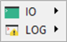
\includegraphics[scale=0.8]{./res/menu_r_term_highlighter.png}\\

\begin{scriptsize}
  \begin{tabularx}{\textwidth}{>{\hsize=0.3\hsize}X>{\hsize=0.7\hsize}X}\\
    \hline
    \textbf{Option} & \textbf{Description} \\
    \hline
    IO & \textit{\href{\#menu\_r\_term\_highlighter\_IO}{See options ...}} \\
    LOG & \textit{\href{\#menu\_r\_term\_highlighter\_Log}{See options ...}} \\
    \hline
  \end{tabularx}
\end{scriptsize}

\hypertarget{menu_r_term_highlighter_IO}{}
\subsubsection{Highlighter IO:}\\
\index{R menu!Term highlighter IO}

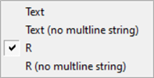
\includegraphics[scale=0.8]{./res/menu_r_term_highlighter_io.png}\\

\begin{scriptsize}
  \begin{tabularx}{\textwidth}{>{\hsize=0.3\hsize}X>{\hsize=0.7\hsize}X}\\
    \hline
    \textbf{Option} & \textbf{Description} \\
    \hline
    Text & Sets the IO highlighter to Text \\
    Text (no multline string) & Sets the IO highlighter to Text without string multline suport \\
    R & Sets the IO highlighter to R \\
    R (no multline string) & Sets the IO highlighter to R without string multline suport \\
    \hline
  \end{tabularx}
\end{scriptsize}

\hypertarget{menu_r_term_highlighter_Log}{}
\subsubsection{Highlighter LOG:}\\
\index{R menu!Term highlighter LOG}

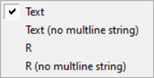
\includegraphics[scale=0.8]{./res/menu_r_term_highlighter_log.png}\\

\begin{scriptsize}
  \begin{tabularx}{\textwidth}{>{\hsize=0.3\hsize}X>{\hsize=0.7\hsize}X}\\
    \hline
    \textbf{Option} & \textbf{Description} \\
    \hline
    Text & Sets the LOG highlighter to Text \\
    Text (no multline string) & Sets the LOG highlighter to Text without string multline suport \\
    R & Sets the LOG highlighter to R \\
    R (no multline string) & Sets the LOG highlighter to R without string multline suport \\
    \hline
  \end{tabularx}
\end{scriptsize}

%\newpage
\hypertarget{menu_r_term_linewrap}{}
\subsubsection{Line wrap:}\\
\index{R menu!Term line wrap}

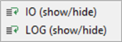
\includegraphics[scale=0.8]{./res/menu_r_term_linewrap.png}\\

\begin{scriptsize}
  \begin{tabularx}{\textwidth}{>{\hsize=0.3\hsize}X>{\hsize=0.7\hsize}X}\\
    \hline
    \textbf{Option} & \textbf{Description} \\
    \hline
    IO & Sets line wrap to IO \\
    LOG & Sets line wrap to LOG \\
    \hline
  \end{tabularx}
\end{scriptsize}

%\hypertarget{menu_r_term_history}{}
\subsubsection{History:}\\
\index{R menu!Term history}

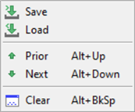
\includegraphics[scale=0.8]{./res/menu_r_term_history.png}\\

\begin{scriptsize}
  \begin{tabularx}{\textwidth}{>{\hsize=0.3\hsize}X>{\hsize=0.7\hsize}X}\\
    \hline
    \textbf{Option} & \textbf{Description} \\
    \hline
    Save & Saves the history \\
    Load & Loads the history \\
    \hdashline[1pt/1pt]
    Prior & Prior section of the history \\
    Next & Next section of the history \\
    \hdashline[1pt/1pt]
    Clear & Clear the Term history \\
    \hline
  \end{tabularx}
\end{scriptsize}

\hypertarget{menu_r_term_workspace}{}
\subsubsection{Workspace:}\\
\index{R menu!Term workspace}

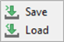
\includegraphics[scale=0.8]{./res/menu_r_term_workspace.png}\\

\begin{scriptsize}
  \begin{tabularx}{\textwidth}{>{\hsize=0.3\hsize}X>{\hsize=0.7\hsize}X}\\
    \hline
    \textbf{Option} & \textbf{Description} \\
    \hline
    Save & Saves the workspace \\
    Load & Loads the workspace \\
    \hline
  \end{tabularx}
\end{scriptsize}

\hypertarget{menu_r_term_fontsize}{}
\subsubsection{Font of active control (not permanent):}\\
\index{R menu!Term fontsize}

\includegraphics[scale=0.8]{./res/menu_fontsize_generic.png}\\

\begin{scriptsize}
  \begin{tabularx}{\textwidth}{>{\hsize=0.3\hsize}X>{\hsize=0.7\hsize}X}\\
    \hline
    \textbf{Option} & \textbf{Description} \\
    \hline
    Increase & Increase the font size \\
    Decrease & Decrease the font size \\
    \hline
  \end{tabularx}
\end{scriptsize}

%\newpage
\hypertarget{menu_r_control_workdir}{}
\subsubsection{Work directory:}\\
\index{Work directory}
\index{getwd()}
\index{setwd()}
\index{R menu!work directory}

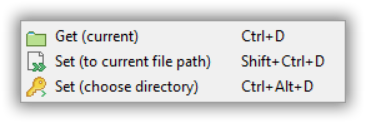
\includegraphics[scale=0.8]{./res/menu_r_control_workdir.png}\\

\begin{scriptsize}
  \begin{tabularx}{\headwidth}{>{\hsize=0.2\hsize}X>{\hsize=0.7\hsize}X}\\
    \hline
    \textbf{Option} & \textbf{Description} \\
    \hline
    Get (current) & Get the work directory of the R interpreter \\
    Set (to current file path) & Set the work directory of the R interpreter to the current file path \\
    Set (choose) & Set the work directory of the R interpreter allowing to choose from the Windows dialog \\
    \hline
  \end{tabularx}
\end{scriptsize}

